\cleardoublepage
\chapter{Conclusiones y trabajos futuros}
\label{chap:conclusiones-trabajos-futuros}

\section{Comparativa lanzamiento ATQ vs tradicional}

\section{Ampliaci�n del Middleware}

\subsection{Sistemas Operativos Windows}

La integraci�n completa con Sistemas Operativos Windows a�n no es posible, ya que las im�genes de ATQ para un despliegue basado en stacks de Swarm y del descubrimiento de servicios, est�n basados en im�genes linux, como CentOS 7\footnote{https://centos.org} o Alpine Linux\footnote{https://alpinelinux.org}. Esto implica que no se pueda desplegar ATQ en sistemas Windows que utilicen contenedores Windows nativos, aunque s� deber�a poderse desplegar ATQ sobre sistemas Windows que operen con contenedores Linux.\newline

Para ello, ser�a necesario crear im�genes espec�ficas con los binarios de ATQ y del descubridor de servicios con una imagen de contenedor basada en Windows como \textit{nanoserver}\footnote{https://hub.docker.com/r/microsoft/nanoserver/}.

\subsection{Integraci�n con Jenkins}

Por otro lado, se podr�a ampliar el proyecto creando un plugin espec�fico para Jenkins para poder as� definir de una manera declarativa sencilla los par�metros para una ejecuci�n el�stica de test de carga usando el middleware ATQ.

\subsection{Soluci�n comercial}

Una soluci�n empresarial ser�a posible creando un portal web con una serie de caracter�sticas como autenticaci�n con Kerberos o LDAP y multi-tenancy de usuarios para poder as� ofrecer una soluci�n SAAS de la herramienta y ofrecerla a trav�s de alg�n tipo de suscripci�n.\newline

Para ello ser�a necesario desplegar ATQ sobre una infraestructura cloud como Amazon Web Services\footnote{https://aws.amazon.com}, Azure\footnote{https://azure.microsoft.com} o Google Cloud Platform\footnote{https://cloud.google.com} usando el orquestador Kubernetes\footnote{https://kubernetes.io} con el objetivo de poder escalar de una manera sencilla la infraestructura en base a la demanda de los usuarios.\clearpage

Una posible arquitectura ser�a la siguiente:

\begin{figure}[h]
    \centering
    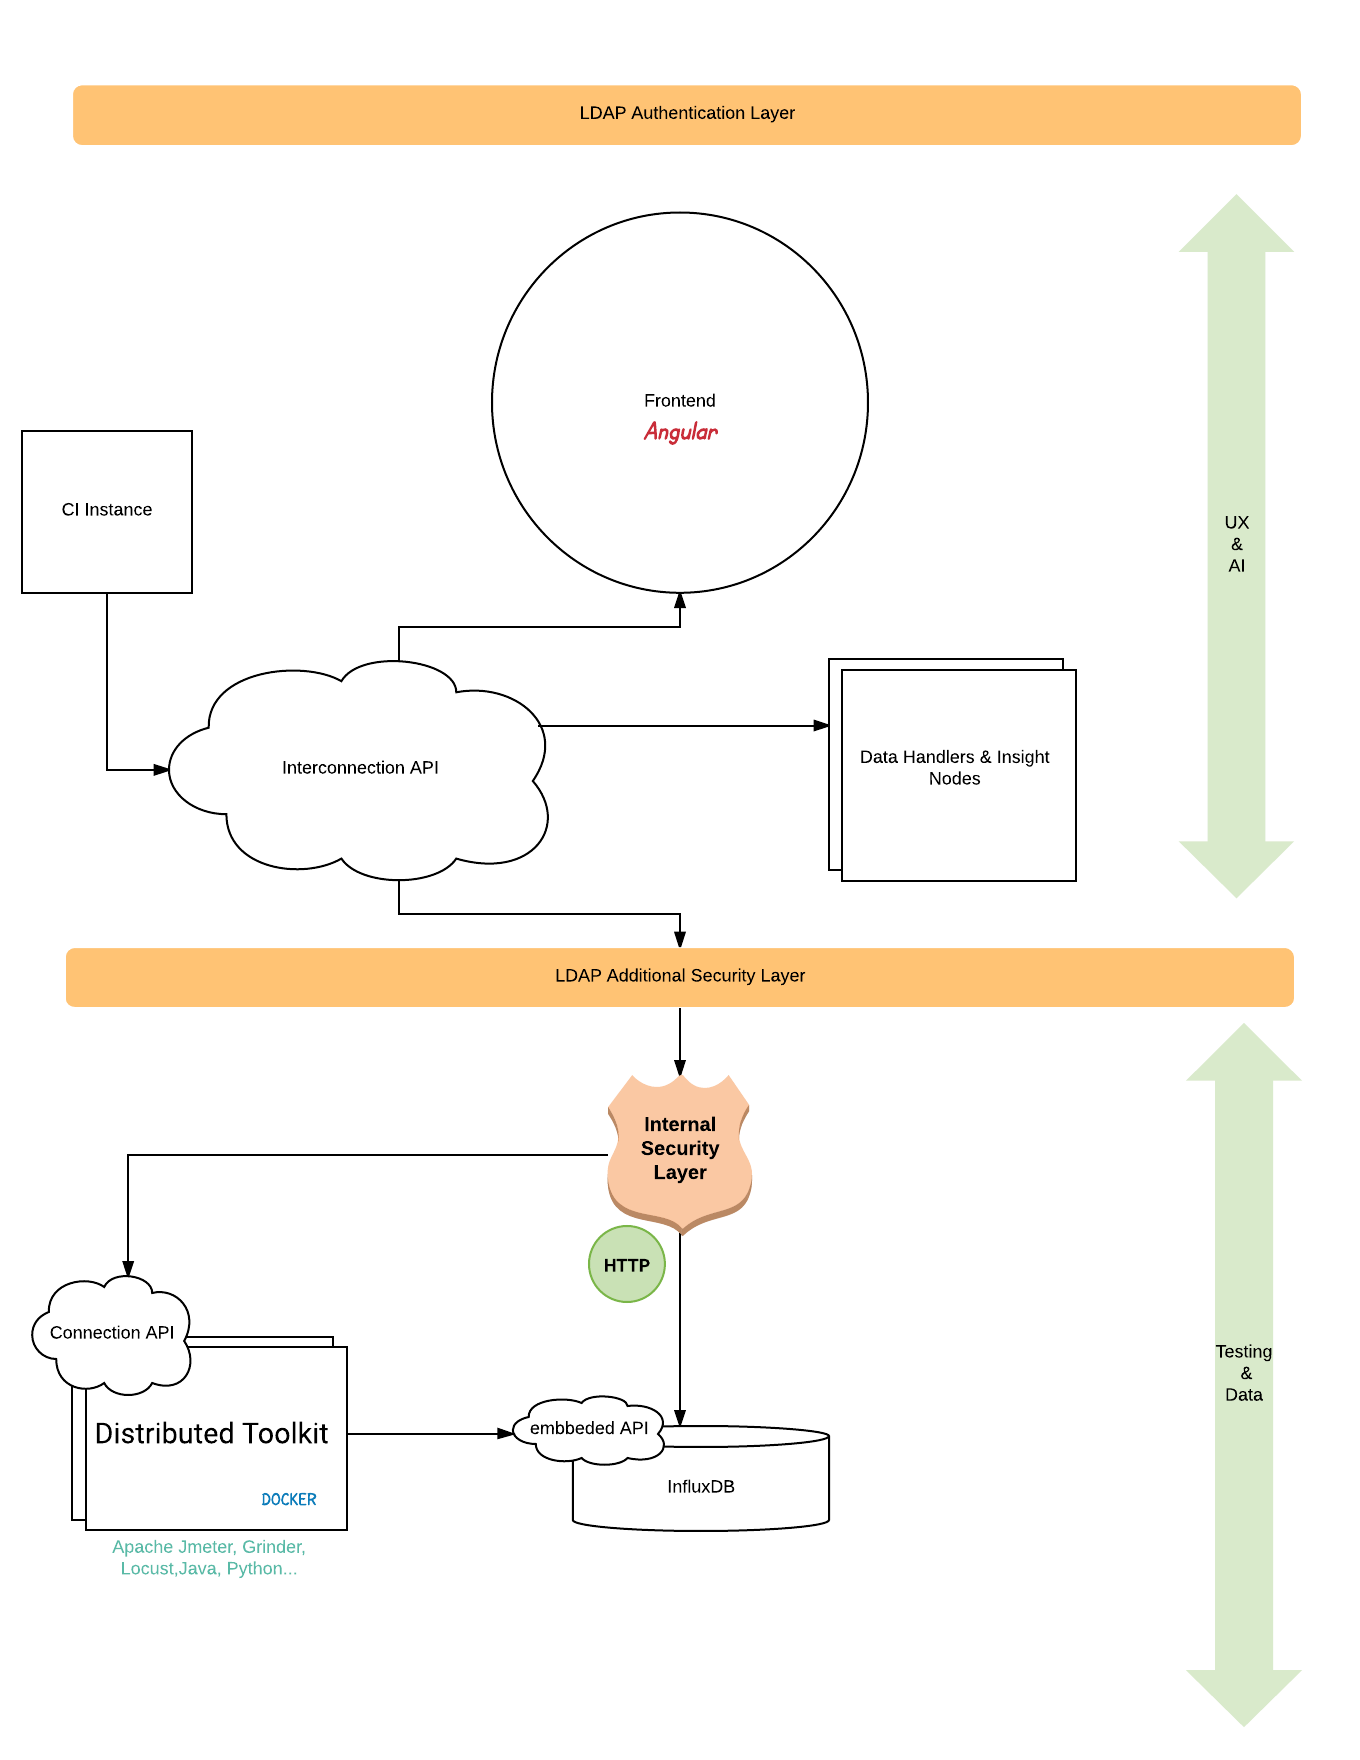
\includegraphics[width=0.8\textwidth]{saas_arch}
    \caption{Arquitectura posible para una soluci�n comercial SAAS}
    \label{fig:saas_arch}
\end{figure}
